\documentclass[11pt, a4paper, onecolumn, oneside]{article}
\usepackage{graphicx}
\usepackage{mathtools}
\renewcommand{\thesection}{\Roman{section}}
\renewcommand{\thesubsection}{\Alph{subsection}.} 

\begin{document}
\title{POLSAR Image Classification via Clustering-WAE Classification Model}
\author{WEN XIE\\
Key Laboratory of Electronic Information Processing\\ for Applications in Scene Investigation\\
Ministry of Public Security\\
Xi’an University of Posts and Telecommunications\\
Xi’an, China \and \\
ZIWEI XIE\\
School of Automation and Information Engineering\\
Xi’an University of Technology\\
Xi’an, China \and \\
FENG ZHAO\\
Key Laboratory of Electronic Information Processing\\ for Applications in Scene Investigation\\
Ministry of Public Security\\
Xi’an University of Posts and Telecommunications\\
Xi’an, China\and \\
Bo Ren\\
School of Artificial Intelligence\\
Xidian University\\
Xi’an, China}

\maketitle

\begin{abstract}
Considering the clustering algorithms could explore the label information automatically, this paper proposes a new method in terms of polarimetric synthetic aperture radar (POLSAR) image classification, which named a clustering-wishart-auto-encoder (WAE) classification model. With considering the statistical distribution characteristic of the POLSAR image, the WAE classification model, which proposed by ourselves, could improve the classification performance of the POLSAR image to some extent. The clustering-WAE classification model, that embedded the K-means clustering algorithm into the objective function of the WAE model, has the ability to improve the network performance. Our proposed method could minimize the difference of intra-class data and maximize the difference of inter-class data, from which the obtained POLSAR image features will be more compact to their corresponding cluster centers. Via simultaneously considering the compactness and statistical distribution of data, our method is capable of improving the POLSAR image classification results. The effectiveness of our proposed classification model has been demonstrated on four real POLSAR data sets.
\end{abstract}

\section{Introduction}

POLSAR (polarimetric synthetic aperture radar) is a kind of multi-channel and multi-parameter imaging radar system. The measured POLSAR data are obtained through transmitting and receiving electromagnetic waves in different polarimetric states \cite{a, b}. With its all-weather, all-time capabilities, radar system been widely applied in the field of remote sensing including terrain classification, target recognition, target detection \cite{c, d, e, f} and so on. POLSAR image terrain classification has become a hot research field of remote sensing image in recent years. During the past decade, lots of POLSAR image classification methods have been proposed, mainly includes three categories which are polarimetric target decomposition \cite{g, h, i}, statistical distribution \cite{j, k} and machine learning \cite{m, n}.\\

The first method, which is based on polarimetric target decomposition, decomposes polarimetric data (such as polarization coherence matrix and covariance matrix) into different components, which are used as structure information and scattering properties of targets. The quite famous methods including Freeman, Cloude, Krogager decomposition and so on \cite{g, h, o}. The second method has been highlighted by many researchers, because of its specially statistical distribution. With multiplicative noise, the statistical distribution of POLSAR image is different from natural images, and has been proved that obey complex gaussian distribution, complex Wishart distribution or others \cite{j, k}. In recent years, many classification methods of machine learning are applied on POLSAR image, for instance, NNs (Neural Networks), SRC (Sparse Representation Classifier), AE (Auto-Encoder) and so on \cite{p, q, r, s}. Many of the machine learning methods are well used in natural image classification instead of POLSAR image, because they do not consider the data characteristic and statistical distribution of POLSAR image. It will be unreasonable when the machine learning methods are applied in POLSAR image directly.\\

Considering the Wishart distribution is one of the most widely used distribution, we proposed the WAE (Wishart-Auto-Encoder) classification model \cite{c} which based on AE network \cite{t}, and has been applied in the field of POLSAR image classification successfully. The WAE network takes the polarization coherency matrix as its input and uses Wishart distance to compute the error between the input and the output. With considering the Wishart distribution of POLSAR data into the optimization procedure of AE network, our proposed WAE classification model is more suitable for processing POLSAR data compared with AE. It could greatly improve the classification accuracy and network performance.\\

The aim of AE network is to minimize the network reconstruction error. Although the WAE classification model fully takes into consideration the statistical distribution of POLSAR data and improves the classification performance, it does not improve the compact of classification features. The objective function of WAE network is to minimize the distance between the input and the output rather than improving the classification ability of model. To make it more suitable for image classification, there are researchers proposed the idea that embedding the K-means algorithm into the AE network in order to improve its discriminative ability \cite{u}, which contains two parts: the reconstruction error, and the distance between the hidden representations and their corresponding cluster centers. With embedding the clustering idea of K-means, the optimized network could increase the inter class differences and decrease the intra class differences of classification features simultaneously. Thus, the hidden representations and clustering centers are updated iteratively during optimization. What is more, the method proposed by literature \cite{u} and \cite{v} have not been used in POLSAR image classification. With considering the statistical distribution of POLSAR image, this paper proposes the Clustering-WAE classification model which based on the above theoretical basis. Results by the test of real POLSAR images show that the proposed method could improve classification performance.\\

The rest of this paper is organized as follows. In Section \ref{sec:two}, the idea of AE based data clustering and WAE classification model are briefly presented. Details about the Clustering-WAE classification model are provided in Section \ref{sec:three}. Four experiment results and discussions are presented in Section \ref{sec:four}. Finally, the conclusion and future works are discussed in Section \ref{sec:five}.

\section{Background Introduction} \label{sec:two}
\subsection{Brief Introduction on WAE Classification Model}

AE network, which has been successfully applied in the field of image features extraction and terrain classification \cite{w, x}, consists of an encoder and a decoder. The goal of AE network is to decrease the network reconstruction error. The F-norm, which is more suitable for natural image rather than POLSAR image \cite{y}, is used to measure the distance of the data in the encoder and the represents in the decoder. In \cite{c}, we proposed WAE classification model consists of a WAE network and a Softmax classifier \cite{z}. For WAE network, the Wishart distance is used as the measurement method in its objection function. We replace the F-norm with Wishart distance for the reason that POLSAR data obeys the Wishart distribution in general. Thus, the classification features extracted by WAE network could improve the POLSAR image classification performance.\\

The structure of WAE network is shown in Fig.\ref{fig:one}, which has the same structure to AE network. The xi , hi and yi are the input, the hidden and the output respectively in Fig.\ref{fig:one}. The $W^{(1)}$ and $W^{(2)}$ represent the weight of encoder and decoder respectively. The loss function of WAE network is shown in Eq.(\ref{eq:one}).

\begin{equation} \label{eq:one}
\min \limits _{W,b} \frac {1}{2N}\sum \limits _{i = 1}^{N} {{d_{Wishart}}\left ({ {H\left ({ {y_{i}} }\right ),H\left ({ {x_{i}} }\right )} }\right )}
\end{equation}
where,
\begin{equation} 
{d_{Wishart}}\left ({ {H\left ({ {y_{i}} }\right ),H\left ({ {x_{i}} }\right )} }\right ) =Tr\left ({ {H{{\left ({ {x_{i}} }\right )}^{( - 1)}}H\left ({ {y_{i}} }\right )} }\right ) \!+\! \ln \left |{ {H\left ({ {x_{i}} }\right )} }\right | \notag
\end{equation}

\begin{figure}
\centering
\fbox{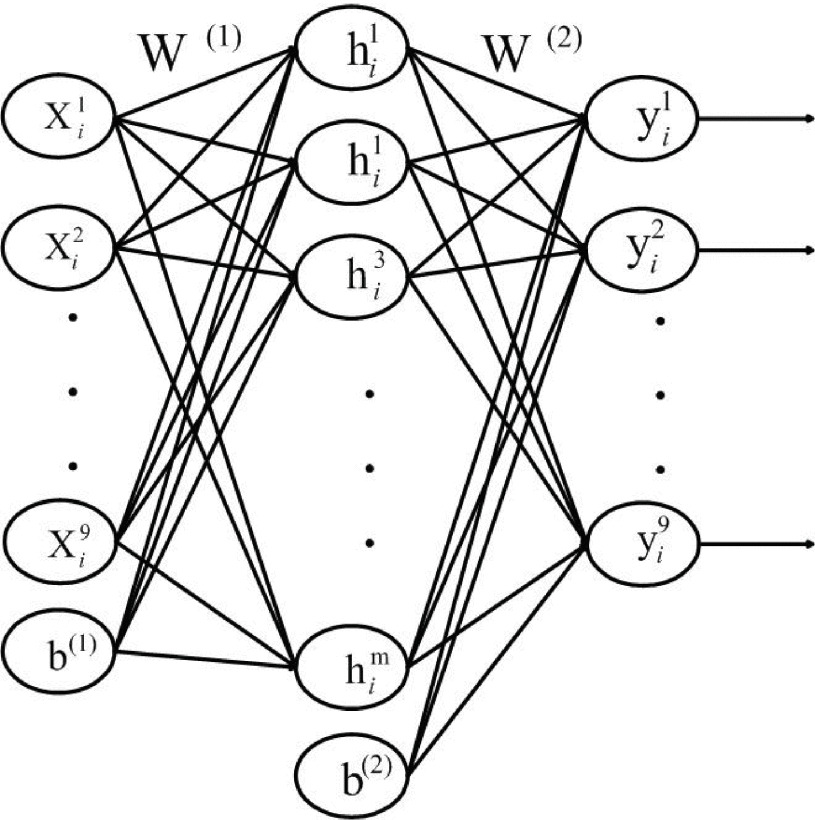
\includegraphics[scale=0.3]{figure_1.jpg}}
\caption{The structure of WAE network.}
\label{fig:one}
\end{figure}

Specifically, a complex coherency matrix, which follows the Wishart distribution, represents a pixel of POLSAR image. The complex coherency matrix is $3\times 3$ , we extract its real and imaginary part respectively, to form a 9-D vector. Then, the input xi and the output yi of WAE network are both a $9-D$ vector. In order to compute the Wishart distance, we use the function $H(\bullet)$ to convert the output $9-D$ vector into the same form as the complex coherency matrix. Thus, in function (\ref{eq:one}), $H(yi)$ and $H(xi)$ are the matrix representation of vector $y_i$ and $x_i$ , $H(x_i)^{(−1)}$ denote the inverse of matrix $H(x_i)$ , and $dWishart(H(y_i),H(x_i))$ is the Wishart distance between $H(y_i)$ and $H(x_i)$ \cite{c}. At last, a Softmax classifier is applied to connect the hidden representations of WAE network to accomplish the POLSAR image classification task.\\

Even though, our WAE classification model has achieved some effects in POLSAR image, the classification features are not very suitable for classification task. Thus, we want to make some change on the network model so as to make the hidden representation more compact.

\subsection{Brief Review on AE Based Data Clustering}

The goal of Data clustering is dividing similar data into the same cluster \cite{u}, which is a essential issue in pattern recognition. K-means \cite{aa, ab}, which is shown in Fig.\ref{fig:two}, is a classical clustering algorithm. The blue snowflakes in Fig.\ref{fig:two}(a) represent all the samples without clustering and the red dot and green dot are the two initialization cluster centers in Fig.\ref{fig:two}(b). Fig.\ref{fig:two}(c) shows the distance between every sample and the cluster centers. On the basis of above distance, Fig.\ref{fig:two}(d)–\ref{fig:two}(f) show the procedure of clustering, and obtain the cluster centers and every sample belongings.

\begin{figure}
\centering
\fbox{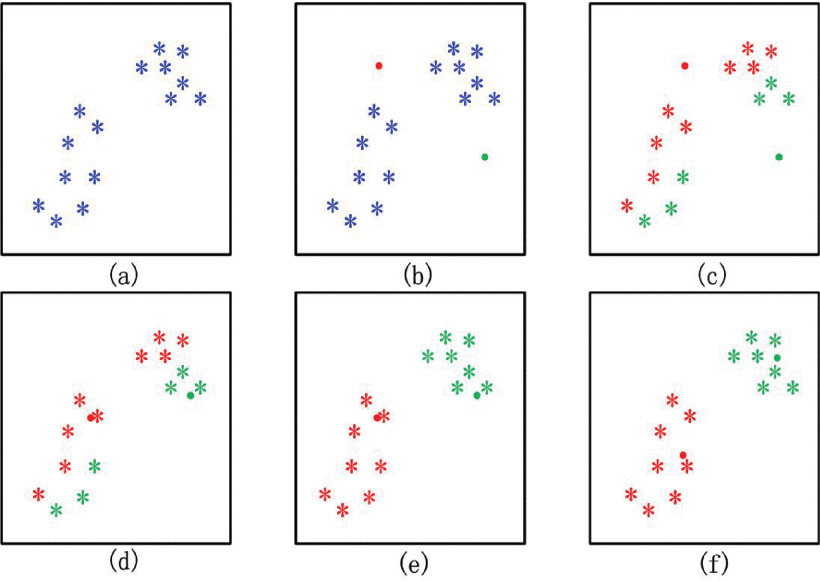
\includegraphics[scale=0.3]{figure_2.jpg}}
\caption{The schematic of K-means algorithm.}
\label{fig:two}
\end{figure}

For the reason that AE network does not require the similar input gain the same representations in the hidden layer, it contributes little to clustering. Thus, \cite{u} proposes a new clustering algorithm that embed K-means into AE network. The Eq.(\ref{eq:two}) is the objective function.

\begin{equation} \label{eq:two}
\begin{split}
\min \limits_{W,b}~\frac {1}{N}\sum \limits _{i = 1}^{N}{{{\left \|{ {x_{i} - {y_{i}}} }\right \|}^{2}}} + \lambda \sum \limits _{i = 1}^{N} {\left \|{ {f^{t}\left ({ {x_{i}} }\right ) - c_{i}^{*}} }\right \|_{F}^{2}} \\
\quad 
\hphantom {\min \limits _{W,b}~}c_{i}^{*} = \arg \min \limits _{c_{j}^{t - 1}} \left \|{ {f^{t}\left ({ {x_{i}} }\right ) - c_{j}^{t - 1}} }\right \|_{F}^{2}
\end{split}
\end{equation}

where $N$ is the number of samples; $f^t(x_i)$ denotes the non-linear mapping function at the tth iteration; $c_j^{t-1}$ is the $j^{th}$ cluster center which computed at the $(t−1)^{th}$ iteration; and $c_i^*$ is the closest cluster center in the hidden layer \cite{u, v}. The Eq.(\ref{eq:two}) makes sure of minimizing reconstruction error of AE network, and meanwhile the hidden data are approximate to their corresponding cluster centers. The cluster centers are optimized by Eq.(\ref{eq:three}).

\begin{equation} \label{eq:three}
c_{j}^{t} = \frac {{\sum \nolimits _{x_{i} \in C_{j}^{t - 1}} {f^{t}\left ({ {x_{i}} }\right )} }}{{\left |{ {C_{j}^{t - 1}} }\right |}}
\end{equation} 

where $c_j^{t-1}$ is the samples belonging to the jth cluster at the $(t−1)^{th}$ iteration, $|C_j|$ denotes the number of samples in this cluster. With optimizing Eq.(\ref{eq:two}) and Eq.(\ref{eq:three}) alternately, the cluster centers and network weights are both updated. Finally, the authors use the obtained cluster centers and optimized AE network to clustering each sample, which is an unsupervised procedure.

Reference \cite{u} is first to combine AE network with clustering, which could acquire a stable and compact hidden representations. Even though the effectiveness of the proposed method has been demonstrated, the experimental datasets are all the natural images. Thus, in this paper, we combine the WAE classification model with the idea of \cite{u}, and propose a new classification model named Clustering-WAE. With considering the POLSAR statistical distribution and hidden representation clustering simultaneously, the Clustering-WAE classification model could improve the classification results of POLSAR image.

\section{Clustering-WAE Classification Model} \label{sec:three}

WAE classification model does not have the ability of minimizing the difference of intra-class of feature representations, and the method of literature \cite{u} has not been used in POLSAR image classification, but the clustering-WAE classification model, which proposed by this paper, combines the advantages of above two methods. The Clustering-WAE classification model not only improves the classification features but also increases the classification results of POLSAR image. We use the coherency matrix vectorization as the input of clustering-WAE which is showing in Eq.(\ref{eq:four}).

\begin{equation} \label{eq:four}
\begin{split}
\langle T_i\rangle =\left[{ {\begin{array}{*{20}{c}} {T_{i}^{11}}& {T_{i}^{12}}& {T_{i}^{13}}\\ {T_{i}^{21}}& {T_{i}^{22}}& {T_{i}^{23}}\\ {T_{i}^{31}}& {T_{i}^{32}}& {T_{i}^{33}} \end{array}} }\right] \\
\to&{x_{i}} = \left [{ {x_{i}^{1},x_{i}^{2},x_{i}^{3},x_{i}^{4},x_{i}^{5},x_{i}^{6},x_{i}^{7},x_{i}^{8},x_{i}^{9}} }\right ]
\end{split}
\end{equation}

where $T_i$ represent the coherency matrix of POLSAR data; $x_i$ is the vectorization vector.

The framework of our proposed model is shown in Fig.\ref{eq:four}, which the $W^{(1)}$ and $W^{(2)}$ are the weights of encoder and decoder respectively. The contents in the green box is the Clustering-WAE network, and the outside is the supervised classifier. From the Fig.\ref{eq:four}, we can see that the three category samples, which are signed by red, blue and green dots, move to their own class gradually with the number of iterations $t$ increasing.

\begin{figure}
\centering
\fbox{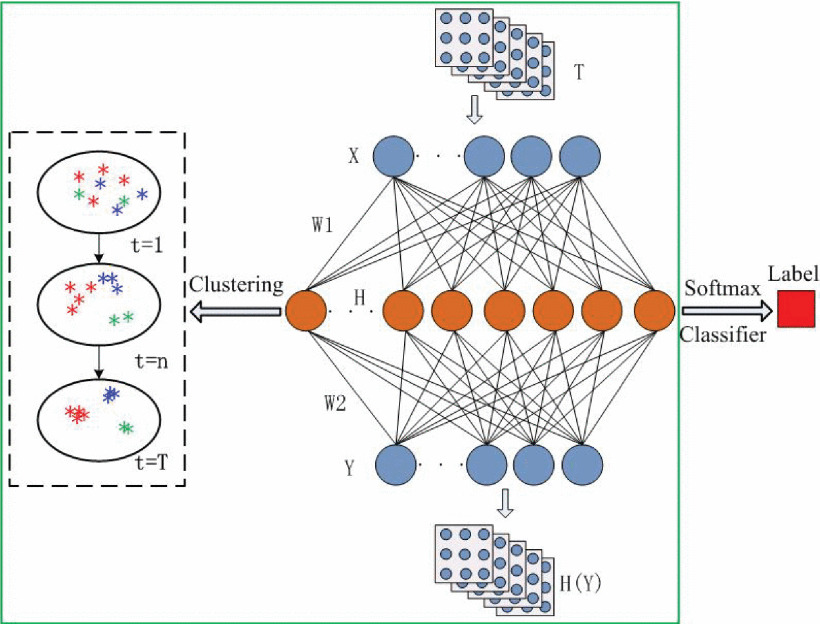
\includegraphics[scale=0.3]{figure_3.jpg}}
\caption{Framework of the our proposed method.}
\label{fig:three}
\end{figure}

The objective function of Clustering-WAE network, which embedding the clustering idea into the WAE network, is shown in the following.

\begin{equation} \label{eq:five}
\begin{split}
\min \limits _{W,b}~\frac {1}{2N}\sum \limits _{i = 1}^{N} {{d_{Wishart}}\left ({ {H\left ({ {y_{i}} }\right ),H\left ({ {x_{i}} }\right )} }\right )} \! \!+\! \!\lambda \sum \limits _{i = 1}^{N} {\left \|{ {h_{i}^{t} - c_{i}^{*}} }\right \|_{F}^{2}} \\
\hphantom {\min \limits _{W,b}~}c_{i}^{*} = \arg \min \limits _{c_{j}^{t - 1}} \left \|{ {h_{i}^{t} - c_{j}^{t - 1}} }\right \|_{F}^{2}
\end{split}
\end{equation}
\begin{equation} \label{eq:six}
\hphantom {\min \limits _{W,b}~}c_{j}^{t} = \frac {{\sum \nolimits _{x_{i} \in C_{j}^{t - 1}} {h_{i}^{t}} }}{{\left |{ {C_{j}^{t - 1}} }\right |}}
\end{equation}

where $N$ is the number of samples; $dWishart(H(y_i),H(x_i))$ represents the Wishart distance between $H(x_i)$ and $H(y_i)$ ; hti is the hidden representation at the tth iteration; $c_i^*$ denotes the closest cluster center of the ith sample in hidden layer; $c_j^{t-1}$ is the jth cluster center computed at the $(t-1)^{th}$ iteration; and $∣∣C_j^{t-1}∣∣$ is the number of samples in the $j^{th}$ cluster center at the $(t-1)^{th}$ iteration. \\

The Eq.(\ref{eq:five}) is composed of two parts, a WAE network and a hidden clustering function, thus, there are two components need to be optimized: the network weights and the cluster centers. Firstly, we randomly initialize the WAE network weights to obtain the hidden representation of training sample. Then, we randomly choose 1\% training sample to initialize the cluster center $C^0$ , and to compute the second function of Eq.(\ref{eq:five}). Finally, we alternately optimize the Eq.(\ref{eq:five}) and Eq.(\ref{eq:six}) to accomplish the optimization process. In Eq.(\ref{eq:five}), we keep the cluster center fixed to optimize the network weights, and then fix the network weights to update the cluster center in Eq.(\ref{eq:six}). \\

The above objective function is the optimization process of Clustering-WAE network which is shown in the green box of Fig.\ref{eq:three}. After this, with the optimization of Clustering-WAE network, we could get the hidden representations of samples, which is used as the classification features of POLSAR image. We apply a Softmax classifier \cite{z} to accomplish the POLSAR image classification task. The objective function of Softmax classifier is presented in Eq.(\ref{eq:seven}). The Softmax classifier, which is a supervised learning method, generalizes logistic regression to classification problems where the predicted label could take on more than one possible values.

\begin{equation} \label{eq:seven}
P\left ({ {l = j|{h_{i}};\theta } }\right ) = \frac {{{\exp ^{h_{i}^{T}{\theta _{j}}}}}}{{\sum \nolimits _{k = 1}^{K} {{\exp ^{h_{i}^{T}{\theta _{k}}}}} }}
\end{equation}

where $j$ is the category being evaluated currently, $h_i$ is the sample, $K$ is the class number, and $\theta$ is the classifier weights. \\

At a word, classification features of the testing samples, which extracted by Clustering-WAE network, are taken as the input of Softmax classifier, finally, the predicted label of POLSAR image are obtained. To facilitate introducing the detail of Clustering-WAE classification model, we conclude it in Table\ref{tab:one}.

\begin{table}
  \caption{Detailed Steps of Algorithm 1}
  \label{tab:one}
  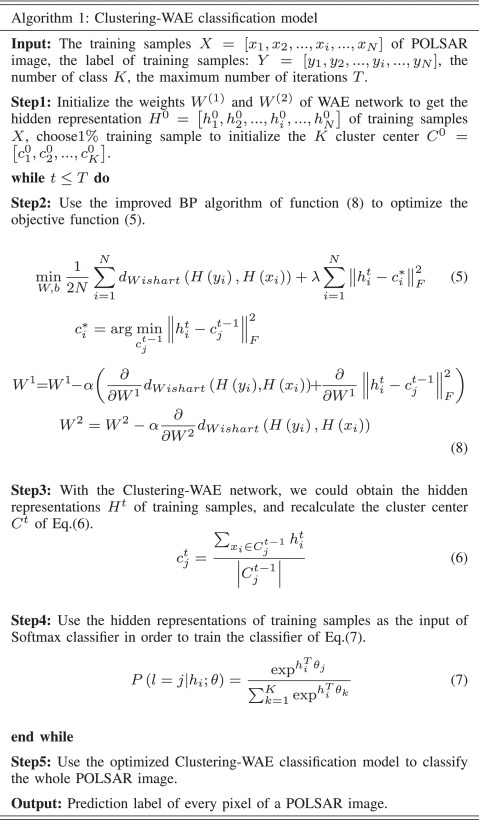
\includegraphics[width=\linewidth]{table_1.jpg}
\end{table}

\section{Experiment and Analysis} \label{sec:four}

In order to verify the effectiveness of Clustering-WAE classification model, several POLSAR datasets are used, including Flevoland farmland, Xi’an area, ESAR, and San Francisco bay. The details of each POLSAR dataset will be introduced in every experimental section. In the experiments, Clustering-WAE method is compared with four methods, including supervised K-means \cite{ac, ad}, supervised Wishart method \cite{ae, af, ag}, AE classification model \cite{r}, and WAE classification model \cite{c}. \\

The AE and WAE classification model are chosen with the same model parameters, such as the size of hidden layers and sparsity which has been discussed in \cite{c}. What is more, the experimental parameters of Clustering-WAE classification model are set the same as WAE classification model, except for the part of hidden layer clustering. In addition, we choose 1\% training samples to initialize the cluster centers of supervised K-means, supervised Wishart and Clustering-WAE classification model. For AE, WAE, and Clustering-WAE classification model, 1\% samples (no matter labeled or unlabeled) are chosen for the purpose of training network, and 5\% labeled samples are chosen to train classifier and fine tuning the whole network model. Thus, the 95\% samples of rest are used for testing. What is more, the iteration number of supervised K-means and Wishart method is set as one, because their cluster centers are initialized by labeled samples and higher classification accuracy is achieved when the iteration number is one [33]. All the experiments are accomplished on the software of MATLAB, conducted on a 3.20-GHz computer with 4.00-GB RAM and repeated 50 times to calculate an average result.

\subsection{Flevoland Image}

The Flevoland farmland image is obtained from a subset of an L-band, multi-look POLSAR data, which acquired by the AIRSAR platform on August 16, 1989. Fig.\ref{fig:four} is its Pauli RGB and ground-truth image which including 15 classes with different colors, and its size is 750×1024 \cite{c}.

\begin{figure}
\fbox{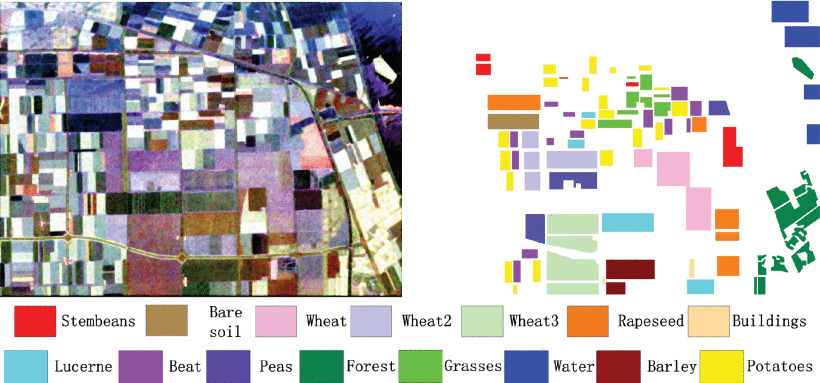
\includegraphics[scale=0.4]{figure_4.jpg}}
\caption{Pauli RGB and ground-truth image of Flevoland.}
\label{fig:four}
\end{figure}

After all the experiment parameters are set up, we conduct experiments on four comparing methods and Clustering-WAE method. The classification results are listed in Table \ref{tab:two} and the highest classification accuracy has been bolded. From Table \ref{tab:two}, we can see that the Clustering-WAE method achieves the highest overall accuracy (OA) value and the Kappa coefficient also obtains improvement in our method. Both of supervised K-means and Wishart classification methods are conducted on the original data of POLSAR, but the OA of Wishart is over nearly 10\% than K-means. The reason is that polarization coherent matrix follows the Wishart statistical distribution. This phenomenon further proves the importance of Wishart distance on measuring POLSAR data, thus our method has very strong pertinence. On the class of water and grasses, the accuracy of Clustering-WAE is improved almost 2\% compared to WAE. Furthermore, with embedding the clustering idea of K-means into WAE, the performance of classification features of Clustering-WAE is improved, including OA and Kappa coefficient.

\begin{table}
  \caption{Classification Performances of Flevoland With Different Methods}
  \label{tab:two}
  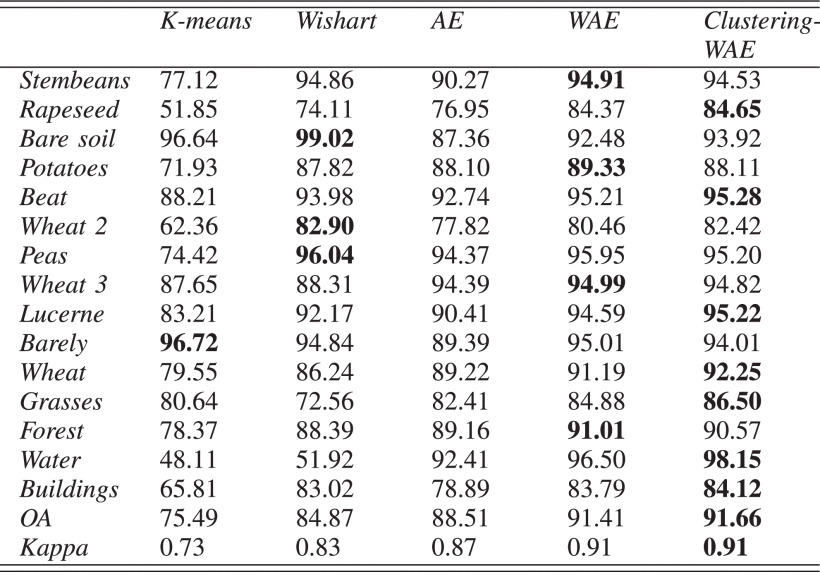
\includegraphics[width=\linewidth]{table_2.jpg}
\end{table}

The classification results of all methods are shown in Fig.\ref{fig:five}. Fig.\ref{fig:five}(a)-(e) represent the different classification models including supervised K-means, supervised Wishart, AE, WAE, and Clustering-WAE. The distinct different results are shown on black ellipse and red rectangle. The grasses in the black ellipse, which is classified much smoother by our proposed method than the others. The water area in the red rectangle, which classified by Clustering-WAE classification model, has less misclassification pixels than the other compared models. From the above, both the accuracy table and classification result figure show that the Clustering-WAE method could improve the classification results, which verify its effectiveness.

\begin{figure}
\fbox{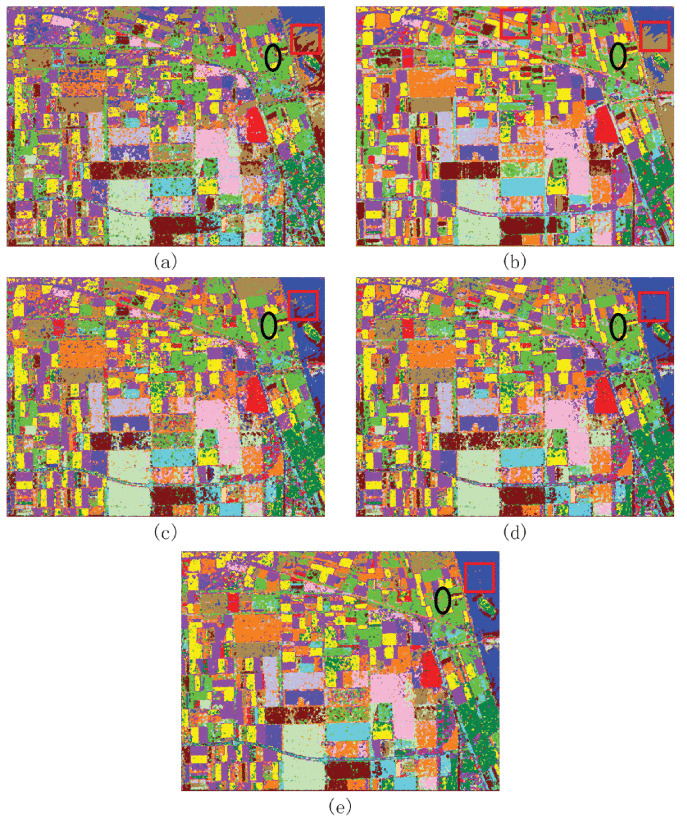
\includegraphics[scale=0.5]{figure_5.jpg}}
\caption{Classification results of different methods: K-means, Wishart, AE, WAE, and Clustering-WAE.}
\label{fig:five}
\end{figure}

\subsection{Xi’an Area Image}

The second dataset is western Xi’an area, China, which acquired by RADARSAT-2. In this experiment, we only choose a block of $512\times 512$ pixels subimage of Xi’an area, because this image is too large. Fig.\ref{fig:six} shows its Pauli RGB and ground-truth image, which including bench land, urban, and river and represented by different colors \cite{c}.


\begin{figure}
\fbox{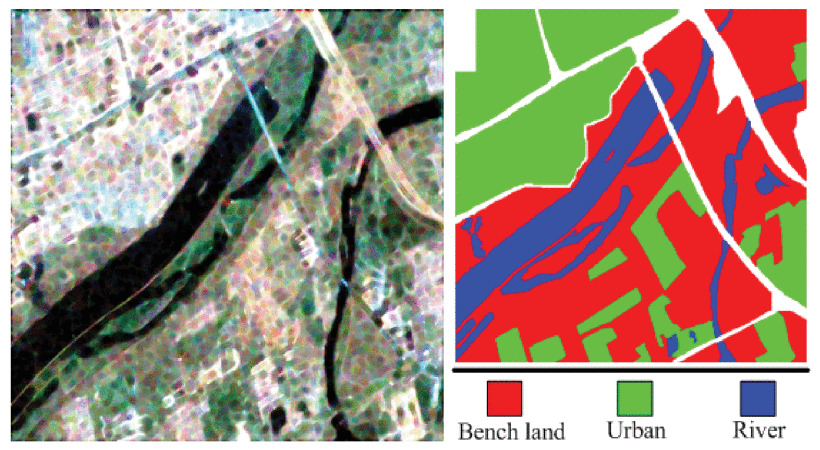
\includegraphics[scale=0.5]{figure_6.jpg}}
\caption{Pauli RGB and ground-truth image of Xi’an.}
\label{fig:six}
\end{figure}

The classification results of our proposed classification model and compared models are shown in Table \ref{tab:three} and Fig.\ref{fig:seven}. Fig.\ref{fig:seven}(a)-(e) represent the different classification methods, respectively. The Clustering-WAE classification model achieves the highest OA and Kappa coefficient, which has been bolded in Table \ref{tab:three}. There are so many misclassification pixels in Fig.\ref{fig:seven}(a), but this situation is improved by Fig.\ref{fig:seven}(b), which shows that Wishart distance is more appropriate toPOLSAR image than F-norm. The distinct different classification results are shown by a black rectangle in Fig.\ref{fig:seven}, such as the urban area of Fig.\ref{fig:seven}(e) is much smoother than the other compared classification methods especially comparedto Fig.\ref{fig:seven}(a).

\begin{table}
  \caption{Classification Performances of Xi’an With Different Methods}
  \label{tab:three}
  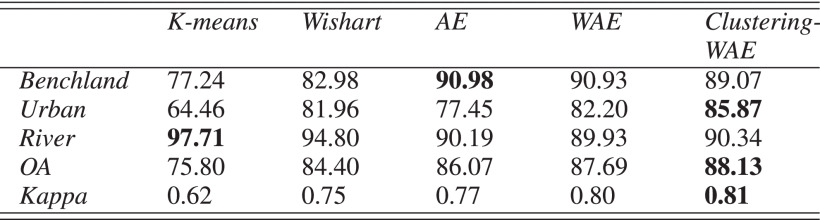
\includegraphics[width=\linewidth]{table_3.jpg}
\end{table}

\begin{figure}
\fbox{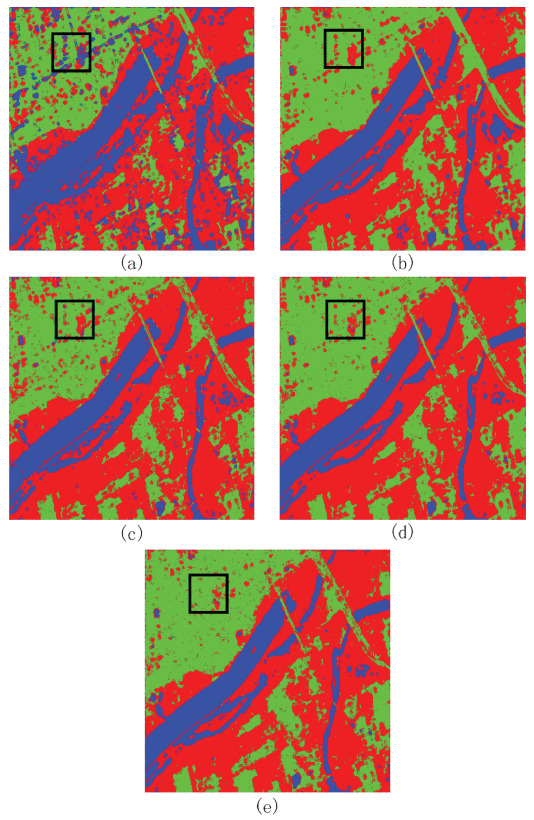
\includegraphics[scale=0.5]{figure_7.jpg}}
\caption{Classification results of different methods: K-means, Wishart, AE, WAE, and Clustering-WAE.}
\label{fig:seven}
\end{figure}

\subsection{ESAR Image}

The ESAR image is obtained from Germany, which is provided by German Aeropave Center \cite{c}. Fig.\ref{fig:eight} shows its Pauli RGB and ground-truth image with the size of $1300\times 1200$. This image is categorized into three kinds including wood land, open area, and Build-up area, which are marked by different colors. The proportion of training samples and the experimental parameters are set the same as the above two experiments. 

\begin{figure}
\fbox{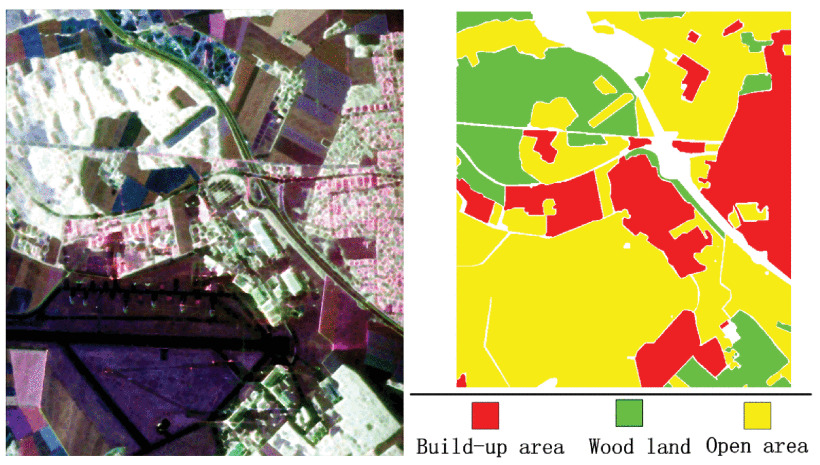
\includegraphics[scale=0.3]{figure_8.jpg}}
\caption{Pauli RGB and ground-truth image of ESAR.}
\label{fig:eight}
\end{figure}

The classification result of every models is displayed in Table \ref{tab:four} and Fig.\ref{fig:nine}. Clustering-WAE classification model achieved the highest OA value and Kappa coefficient. What is more, the classification accuracy of wood land achieves great improvement. Furthermore, we can see that the area in the black rectangle of Fig.\ref{fig:nine}(e) is much smoother than the other compared methods, which gives strong evidence of effectiveness of Clustering-WAE classification model once again.

\begin{table}
  \caption{ Classification Performances of ESAR With Different Methods}
  \label{tab:four}
  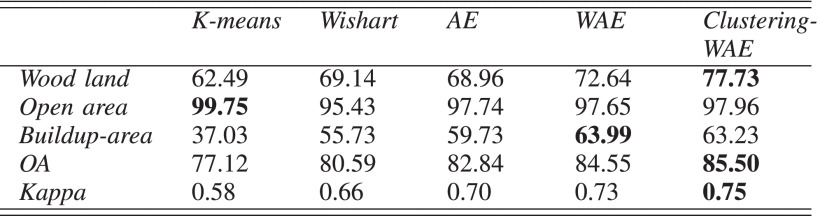
\includegraphics[width=\linewidth]{table_4.jpg}
\end{table}

\begin{figure}
\fbox{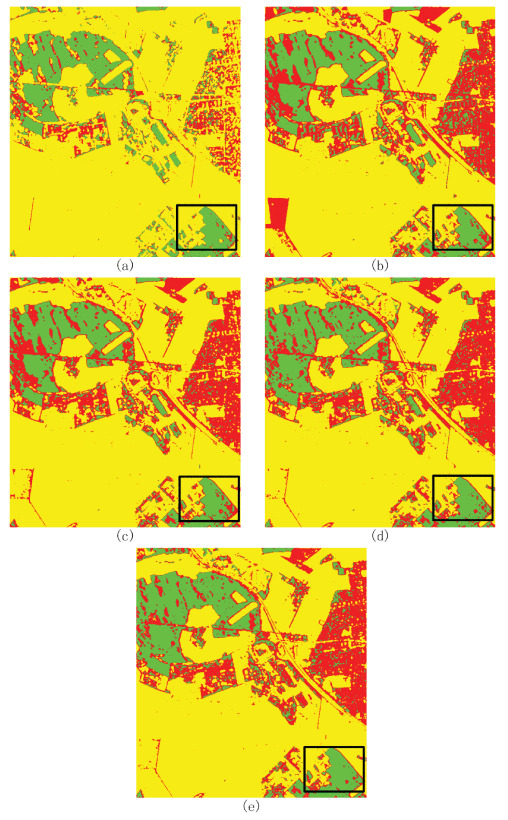
\includegraphics[scale=0.4]{figure_9.jpg}}
\caption{Classification results of different methods: K-means, Wishart, AE, WAE, and Clustering-WAE.}
\label{fig:nine}
\end{figure}

\subsection{San Francisco Image}

The last experimental dataset is San Francisco bay which is obtained by NASA/JPL AIRSAR. The size of this scene is $1895\times 1419$ , which contains five mainly categories, including water, developed, high-density urban, low-density urban, and vegetation \cite{c}. Fig.\ref{fig:ten} is the Pauli RGB and ground-truth image which different colors indicates different classes.

\begin{figure}
\fbox{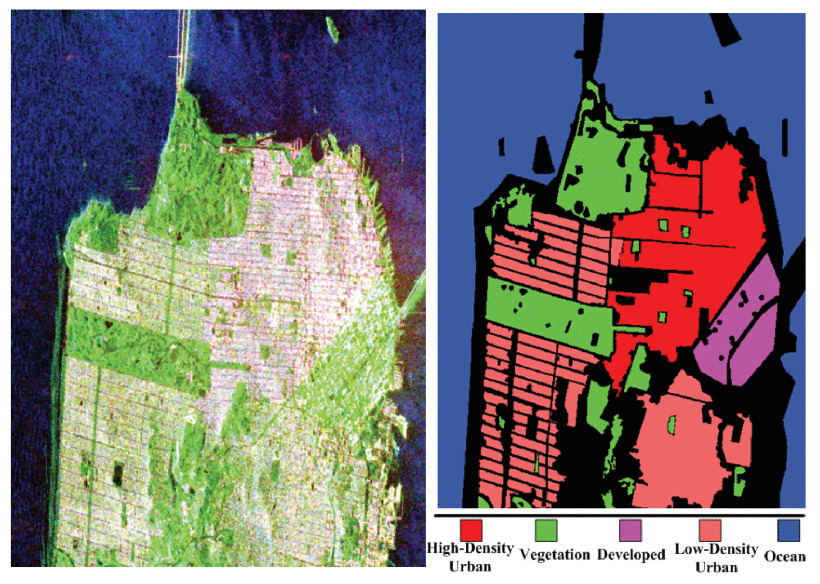
\includegraphics[scale=0.3]{figure_10.jpg}}
\caption{Pauli RGB and ground-truth image of San Francisco.}
\label{fig:ten}
\end{figure}

Table \ref{tab:five} shows the classification accuracies of all classification methods. Our proposed method gets the highest OA and Kappa coefficient, which have increased by more than one percentage point compared to WAE and 20 percentage point to K-means. Especially, the Low-density area of our method appreciates more than 9 percent compared to WAE. Fig.\ref{fig:eleven} also demonstrates the effectiveness of Clustering-WAE classification model. In addition, the classification quality of Fig.\ref{fig:eleven}(e) is smoother than that of Fig.\ref{fig:eleven}(a)-(d), especially in the black rectangle.

\begin{table}
  \caption{ Classification Performances of San Francisco With Different Methods}
  \label{tab:five}
  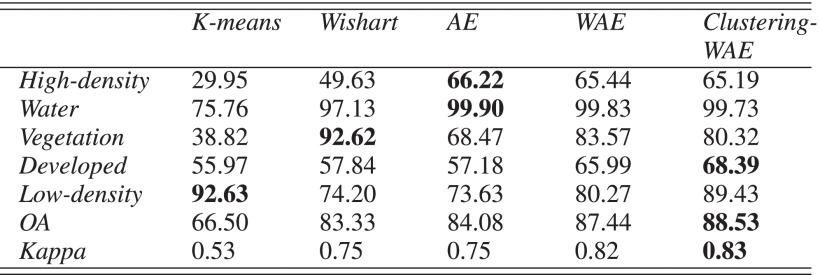
\includegraphics[width=\linewidth]{table_5.jpg}
\end{table}

\begin{figure}
\fbox{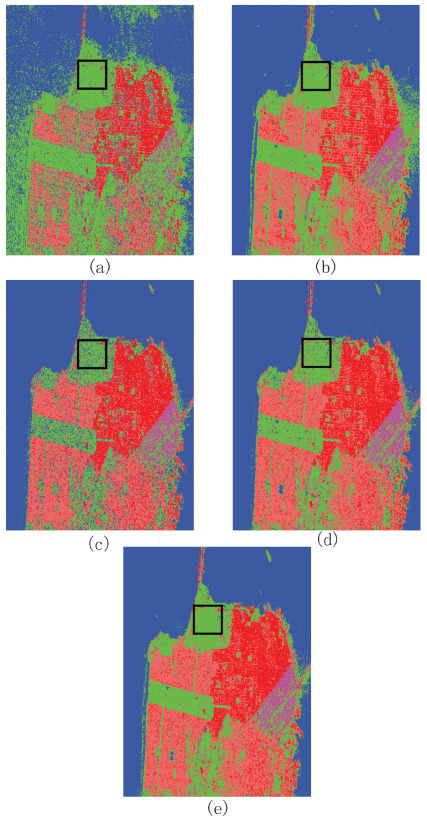
\includegraphics[scale=0.4]{figure_11.jpg}}
\caption{Pauli RGB and ground-truth image of San Francisco.}
\label{fig:eleven}
\end{figure}

\section{Conclusion and Future Work}

In this paper, we have proposed a new classification model, which named Clustering-WAE, to classifying POLSAR image. Considering the statistical distribution of POLSAR data, we combine the idea of clustering and WAE classification model in order to improve the classification result. Our preceding WAE method takes a full account of statistical distribution of POLSAR data, but it does not adding the label information of training samples. Reference \cite{u} makes good use of the K-means and AE network to improve the performance of image classification. Thus, we combine the method of \cite{u} and WAE to construct the Clustering-WAE network, whose hidden representations are clustered during the network optimization procedure. Finally, the Clustering-WAE network is connected to a Softmax classifier to complete the POLSAR image classification task. Experimental results on real POLSAR datasets demonstrate the proposed methods is significantly effective. The Clustering-WAE classification model could achieve impressive classification performance compared to comparison algorithm. Note that the hidden layer in Clustering-WAE classification model is only one, therefore, our future work is researching the deep network in order to extract more valid POLSAR classification features. What is more, researching the statistical distribution of hidden representations is another important research content in our future works.


\begin{thebibliography}{35}
\bibitem{a} F. T. Ulaby, C. Elachi, "Radar polarimetry for geoscience applications", Geocarto Int., vol. 5, pp. 38, 1990.
\bibitem{b} K. Tragl, "Polarimetric radar backscattering from reciprocal random targets", IEEE Trans. Geosci. Remote Sens., vol. 28, no. 5, pp. 856-864, Sep. 1990.

\bibitem{c} 	W. Xie et al., "POLSAR image classification via Wishart-AE model or Wishart-CAE model", IEEE J. Sel. Topics Appl. Earth Observ. Remote Sens., vol. 10, no. 8, pp. 3604-3615, Aug. 2017.

\bibitem{d} 	S. Uhlmann, S. Kiranyaz, "Integrating color features in polarimetric SAR image classification", IEEE Trans. Geosci. Remote Sens., vol. 52, no. 4, pp. 2197-2216, Apr. 2014.

\bibitem{e} 	A. J. Bennett, A. Currie, "Use of high-resolution polarimetric SAR for automatic target recognition", Proc. SPIE, vol. 4727, pp. 146-153, Aug. 2002.

\bibitem{f} C. He, S. Li, Z. Liao, M. Liao, "Texture classification of PolSAR data based on sparse coding of wavelet polarization textons", IEEE Trans. Geosci. Remote Sens., vol. 51, no. 8, pp. 4576-4590, Aug. 2013.

\bibitem{g} 	S. R. Cloude, E. Pottier, "An entropy based classification scheme for land applications of polarimetric SAR", IEEE Trans. Geosci. Remote Sens., vol. 35, no. 1, pp. 68-78, Jan. 1997.

\bibitem{h} A. Freeman, S. L. Durden, "A three-component scattering model for polarimetric SAR data", IEEE Trans. Geosci. Remote Sens., vol. 36, no. 3, pp. 963-973, May 1998.

\bibitem{i} E. Pottier, "Dr. J. R. Huynen’s main contributions in the development of polarimetric radar techniques and how the ’radar targets phenomenological concept’ becomes a theory", Proc. SPIE, vol. 1748, pp. 72-86, Feb. 1993.

\bibitem{j}J. S. Lee, M. R. Grunes, "Classification of multi-look polarimetric SAR data based on complex Wishart distribution", Int. J. Remote Sens., vol. 15, no. 11, pp. 2299-2311, 1992.

\bibitem{k}	W. B. Silva, C. C. Freitas, S. J. S. Sant’Anna, A. C. Frery, "Classification of segments in PolSAR imagery by minimum stochastic distances between Wishart distributions", IEEE J. Sel. Topics Appl. Earth Observ. Remote Sens., vol. 6, no. 3, pp. 1263-1273, Jun. 2013.
W. Xie, L. Jiao, J. Zhao, "PolSAR image classification via D-KSVD and NSCT-domain features extraction", IEEE Geosci. Remote Sens. Lett., vol. 13, no. 2, pp. 227-231, Feb. 2016.

\bibitem{m}	J. Geng, J. Fan, H. Wang, X. Ma, B. Li, F. Chen, "High-resolution SAR image classification via deep convolutional autoencoders", IEEE Trans. Geosci. Remote Sens., vol. 12, no. 11, pp. 2351-2355, Nov. 2015.

\bibitem{n}E. Krogager, "Properties of the sphere diplane helix (target scattering matrix) decomposition", Mol. Ecology, vol. 15, no. 11, pp. 3205-3217, 2006.

\bibitem{o}	Z. Zhang, H. Wang, F. Xu, Y.-Q. Jin, "Complex-valued convolutional neural network and its application in polarimetric SAR image classification", IEEE Trans. Geosci. Remote Sens., vol. 55, no. 12, pp. 7177-7188, Dec. 2017.

\bibitem{p}	S. De, L. Bruzzone, A. Bhattacharya, F. Bovolo, S. Chaudhuri, "A novel technique based on deep learning and a synthetic target database for classification of urban areas in PolSAR data", IEEE J. Sel. Topics Appl. Earth Observ. Remote Sens., vol. 11, no. 1, pp. 154-170, Jan. 2018.

\bibitem{q}Y. Chen, L. Jiao, Y. Li, J. Zhao, "Multilayer projective dictionary pair learning and sparse autoencoder for PolSAR image classification", IEEE Trans. Geosci. Remote Sens., vol. 55, no. 12, pp. 6683-6694, Dec. 2017.

\bibitem{r}C. Lardeux et al., "Support vector machine for multifrequency SAR polarimetric data classification", IEEE Trans. Geosci. Remote Sens., vol. 47, no. 12, pp. 4143-4152, Dec. 2009.

\bibitem{s}D. E. Rumelhart, G. E. Hinton, R. J. Williams, Learning Representations by Back-Propagating Errors, Cambridge, MA, USA:MIT Press, 1988.

\bibitem{t}	C. Song, Y. Huang, F. Liu, Z. Wang, L. Wang, "Deep auto-encoder based clustering", Intell. Data Anal., vol. 18, no. 6S, pp. S65-S76, 2014.

\bibitem{u}C. Song, F. Liu, Y. Huang, L. Wang, T. Tan, "Auto-encoder based data clustering" in Iberoamerican Congress on Pattern Recognition, Berlin, Germany:Springer, vol. 8252, pp. 117-124, 2013.

\bibitem{v}	X. Ma, H. Wang, J. Geng, "Spectral–spatial classification of hyperspectral image based on deep auto-encoder", IEEE J. Sel. Topics Appl. Earth Observ. Remote Sens., vol. 9, no. 9, pp. 4073-4085, Sep. 2016.

\bibitem{w}	F. Lv, M. Han, T. Qiu, "Remote sensing image classification based on ensemble extreme learning machine with stacked autoencoder", IEEE Access, vol. 5, 2017.

\bibitem{x}	H. Permuter, J. Francos, I. Jermyn, "A study of Gaussian mixture models of color and texture features for image classification and segmentation", Pattern Recognit., vol. 39, no. 4, pp. 695-706, 2006.

\bibitem{y}D. Heckerman, C. Meek, "Models and selection criteria for regression and classification", Proc. 13th Conf. Uncertainty Artif. Intell., pp. 223-228, 1997.

\bibitem{z}N. B. Amor, S. Benferhat, Z. Elou	J. A. Hartigan, M. A. Wong, "Algorithm AS 136: A k-means clustering algorithm", Appl. Statist., vol. 28, no. 1, pp. 100-108, 1979.

\bibitem{aa}A. K. Jain, M. N. Murty, P. J. Flynn, "Data clustering: A review", ACM Comput. Surv., vol. 31, no. 3, pp. 264-323, Sep. 1999.

\bibitem{ab}S. H. Al-Harbi, V. J. Rayward-Smith, " Adapting k -means for supervised clustering ", Appl. Intell., vol. 24, no. 3, pp. 219-226, 2006.

\bibitem{ac}S. Okawa, A. Ishigure, M. Sawamura, "An application to a paper classification support by fuzzy K-means", IPSJ SIG Tech. Rep., vol. 2006, pp. 81-84, Dec. 2006.

\bibitem{ad}	J. S. Lee, M. R. Grunes, T. L. Ainsworth, L. J. Du, D. L. Schuler, S. R. Cloude, "Unsupervised classification using polarimetric decomposition and the complex Wishart classifier", IEEE Trans. Geosci. Remote Sens., vol. 37, no. 5, pp. 2249-2258, Sep. 1999.

\bibitem{ae} J. S. Lee, M. R. Grunes, T. L. Ainsworth, L. J. Du, D. L. Schuler, S. R. Cloude, "Unsupervised classification using polarimetric decomposition and complex Wishart classifier", Proc. IEEE Int. Geosci. Remote Sens. Symp., vol. 4, pp. 2178-2180, Jul. 1998.

\bibitem{af}M.-K. Kang, K.-E. Kim, S.-J. Cho, H. Lee, J.-H. Lee, "Wishart supervised classification results of C-band polarimetric GB-SAR image data", Proc. IEEE Int. Geosci. Remote Sens. Symp., pp. 459-462, Jul. 2011.

\bibitem{ag}F. Liu, L. Jiao, B. Hou, S. Yang, "POL-SAR image classification based on Wishart DBN and local spatial information", IEEE Trans. Geosci. Remote Sens., vol. 54, no. 6, pp. 3292-3308, Jun. 2016.
\bibitem{ah}A. Freeman, S. L. Durden, "A three-component scattering model for polarimetric SAR data", IEEE Trans. Geosci. Remote Sens., vol. 36, no. 3, pp. 963-973, May 1998.

\end{thebibliography}

\end{document}